\documentclass[border=4pt,12pt]{standalone}
% House style for redrawn exam diagrams (diagram-v4: 0.4pt lines, filled -latex arrows, fine dashes; stipple and hatching drawn as real dots/lines (no PDF/SVG patterns, so they render in every browser and at any scale); transparent background). Every figure \input's this.
\usepackage{amsmath,amssymb}
\usepackage{txfonts}
\usepackage{pdfrender,xcolor}
% \halo{text}: label on shading. The shading stops just around each letter's outline (a thin knock-out that follows the
% glyphs, like the papers' typesetting), never a box. Owner: "I don't want a box around the text".
\newcommand{\halo}[1]{\leavevmode\rlap{\pdfrender{TextRenderingMode=2,LineWidth=2.2pt,LineJoinStyle=1,StrokeColor=white,FillColor=white}#1}#1}
\usepackage{tikz,pgfplots}
\pgfplotsset{compat=1.18}
\usetikzlibrary{arrows.meta,calc,angles,quotes,patterns,patterns.meta,intersections,positioning,decorations.markings,shapes.geometric}
% Stipple and hatching are drawn as actual dots / lines clipped to the region (path picture), NOT as pattern fills:
% SVG <pattern> fills vanish or blur when browsers scale the image, so the owner could not see the shading.
% Each dot is a 0.72pt square (keeps SVGs small; reads as a dot at print size). Dots sit on one global staggered grid, so neighbouring regions line up.
\makeatletter
\newdimen\ex@x \newdimen\ex@y \newdimen\ex@xa \newdimen\ex@ya \newdimen\ex@xb \newdimen\ex@yb \newcount\ex@row
\def\exam@stipplecolor{black!75}\def\exam@dotr{0.42pt}\def\exam@dotgap{2.5}
\def\ex@rowdots{\ifdim\ex@x<\ex@xb \pgfpathrectangle{\pgfqpoint{\dimexpr\ex@x-0.36pt\relax}{\dimexpr\ex@y-0.36pt\relax}}{\pgfqpoint{0.72pt}{0.72pt}}\advance\ex@x by \exam@dotgap pt\relax\expandafter\ex@rowdots\fi}
\def\exam@stipple{%
  \pgftransformreset% dots are sized in real points even inside scaled pictures
  \pgfpointanchor{path picture bounding box}{south west}\ex@xa=\pgf@x \ex@ya=\pgf@y
  \pgfpointanchor{path picture bounding box}{north east}\ex@xb=\pgf@x \ex@yb=\pgf@y
  \pgfsetfillcolor{\exam@stipplecolor}\pgfmathsetmacro\ex@h{\exam@dotgap/2}%
  \pgfmathtruncatemacro\ex@r{floor(\ex@ya/\ex@h)-1}\ex@row=\ex@r\relax
  \ex@y=\ex@r\dimexpr\ex@h pt\relax
  \loop\ifdim\ex@y<\ex@yb
    \pgfmathtruncatemacro\ex@c{floor(\ex@xa/\exam@dotgap)-1}\ex@x=\ex@c\dimexpr\exam@dotgap pt\relax
    \ifodd\ex@row \advance\ex@x by \ex@h pt\fi
    \ex@rowdots
    \advance\ex@y by \ex@h pt \advance\ex@row by 1
    \ifnum\numexpr\ex@row-(\ex@row/4)*4\relax=0 \pgfusepath{fill}\fi% flush every 4 rows: bounded TeX memory, few clip copies in the SVG
  \repeat\pgfusepath{fill}}
\newdimen\ex@d
\def\exam@hatch#1{% #1 = 1 for /, -1 for \ ; lines 45 degrees, 3pt apart
  \pgftransformreset
  \pgfpointanchor{path picture bounding box}{south west}\ex@xa=\pgf@x \ex@ya=\pgf@y
  \pgfpointanchor{path picture bounding box}{north east}\ex@xb=\pgf@x \ex@yb=\pgf@y
  \ex@d=\dimexpr\ex@yb-\ex@ya\relax \ex@x=\dimexpr\ex@xa-\ex@d\relax
  \loop\ifdim\ex@x<\ex@xb
    \ifnum#1>0 \pgfpathmoveto{\pgfqpoint{\ex@x}{\ex@ya}}\pgfpathlineto{\pgfqpoint{\dimexpr\ex@x+\ex@d\relax}{\ex@yb}}%
    \else \pgfpathmoveto{\pgfqpoint{\ex@x}{\ex@yb}}\pgfpathlineto{\pgfqpoint{\dimexpr\ex@x+\ex@d\relax}{\ex@ya}}\fi
    \advance\ex@x by 4.24pt
  \repeat
  \pgfsetlinewidth{0.4pt}\pgfsetstrokecolor{black}\pgfusepath{stroke}}
\def\examstipple{\exam@stipple}\def\examhatch{\exam@hatch}\def\examsetstipplecolor#1{\def\exam@stipplecolor{#1}}\def\examsetdotgap#1{\def\exam@dotgap{#1}}
\makeatother
% (legacy pattern kept for old files)
% staggered stipple like the NESA papers' dotted shading
\pgfdeclarepatternformonly{exam stipple}{\pgfpointorigin}{\pgfqpoint{2.2pt}{2.2pt}}{\pgfqpoint{2.2pt}{2.2pt}}{%
  \pgfpathcircle{\pgfqpoint{0.55pt}{0.55pt}}{0.42pt}\pgfpathcircle{\pgfqpoint{1.65pt}{1.65pt}}{0.42pt}\pgfusepath{fill}}
\tikzset{
  every picture/.style={line width=0.6pt, >={Latex[length=2mm,width=1.3mm]}},
  curve/.style={line width=0.6pt},
  open arrow/.style={-{Latex[length=2mm,width=1.3mm]}},  % owner: filled -latex heads everywhere, no open chevrons
  aux/.style={dash pattern=on 2pt off 1.5pt, line width=0.6pt},
  shade/.code={\def\exA{#1}\def\exB{none}\ifx\exA\exB\else\pgfkeysalso{fill=black!18}\fi},
  shade/.default=on,
  shade dots/.style={fill=none, path picture={\examstipple}},
  stipple color/.code={\examsetstipplecolor{#1}},
  stipple gap/.code={\examsetdotgap{#1}},
  shade dense dots/.style={fill=none, stipple gap=1.6, path picture={\examstipple}},
  shade hatch/.style={fill=none, path picture={\examhatch{1}}},
  shade hatch reverse/.style={fill=none, path picture={\examhatch{-1}}},
  shade solid/.style={fill=black},
  pt/.style={circle, fill, inner sep=1.1pt},
  open pt/.style={circle, draw, fill=white, inner sep=1.1pt},
}
\pgfplotsset{
  exam axes/.style={axis lines=middle, axis line style={->}, xlabel={$x$}, ylabel={$y$},
    xlabel style={anchor=west}, ylabel style={anchor=south}, tick label style={font=\small},
    every axis plot/.append style={line width=0.6pt, black}, samples=200, clip=false,
    enlargelimits=false, axis on top},
}

\begin{document}
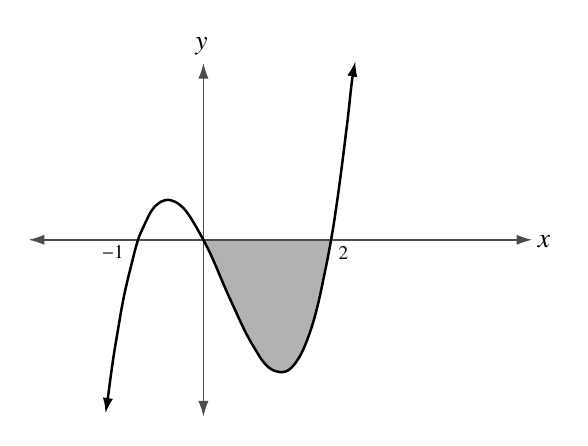
\begin{tikzpicture}[x=0.0127cm,y=-0.0127cm]
  % shaded region between the curve and the x-axis, x = 0 to 2 (mid grey in the crop, drawn lighter)
  \fill[black!30] plot[smooth] coordinates {(198,237) (200.6,242) (203.1,247) (205.5,252.2) (207.8,257.4) (210.1,262.7) (212.4,268.1) (214.7,273.4) (217,278.8) (219.3,284.2) (221.6,289.4) (223.9,294.4) (226.2,299.5) (228.5,304.5) (230.7,309.4) (232.9,314.3) (235,319.1) (237,323.7) (239.6,328.3) (242.2,332.9) (244.4,337.6) (246.7,341.8) (249.6,346.6) (252.4,351.1) (255.7,355.7) (258.8,359.9) (261.9,363.4) (265.1,366.1) (268.4,368) (272,369.2) (275.5,369.7) (278.8,369.4) (281.7,368.3) (284.6,366.4) (287.6,363.3) (290.5,359.6) (293.2,355.4) (295.7,350.7) (298.2,345.7) (300.5,340.8) (302.5,335.7) (304.3,330.8) (305.8,325.5) (307.4,320.4) (309.1,315.5) (310.3,311) (311.5,305.5) (312.6,300.1) (313.8,295) (315.4,289.8) (316.7,284.8) (317.5,279.7) (318.4,274) (319.4,268.5) (320.5,263.1) (321.8,257.7) (323.2,252.1) (324.4,246.9) (325.2,241.8) (325.6,237)} -- cycle;
  \draw[black!70,<->] (23,237) -- (527,237);
  \draw[black!70,<->] (198,414) -- (198,60);
  \node at (538,239) {$x$};
  \node at (196,43) {$y$};
  \node[font=\scriptsize,anchor=north east,inner sep=1pt] at (122,239) {$-1$};
  \node[font=\scriptsize] at (338,250) {$2$};
  \draw[<->, line width=0.9pt] plot[smooth] coordinates {(100,411) (102.3,395.9) (104.3,380.7) (106.4,365.4) (108.6,350.3) (111.1,335.3) (113.7,319.9) (116.3,304.7) (119.2,290.1) (122.5,275.7) (126.2,260.8) (130,245.8) (133.8,233.5) (139.1,221.7) (144.7,210.2) (149.7,203.4) (155.4,199) (160.8,197.2) (165.8,197.6) (171.9,200.2) (178.2,205.5) (184.5,213.8) (191.8,226) (198.9,238.8) (205.2,251.5) (211.2,265.1) (217.2,279.4) (223.2,293.1) (229.6,307) (235.9,320.8) (242,333.1) (249.2,345.6) (256.3,357) (262.3,363.9) (268.2,367.7) (274.5,369.3) (279.8,368.9) (284.2,366.6) (289.6,360.9) (295.6,351.4) (300.8,339.8) (305.5,326.8) (309.6,313.2) (313.2,299) (316.4,284.3) (319.5,269.3) (322.6,254) (325.3,239.2) (327.9,224.2) (330.2,208.9) (332.4,193.8) (334.5,178.4) (336.5,163.1) (338.5,147.4) (340.4,131.9) (342.3,116.6) (344,101.3) (345.6,86.17) (347.5,71.65) (350,58)};
\end{tikzpicture}
\end{document}
